\chapter{MONWES}
\label{capitolo3}
\thispagestyle{empty}
\vspace{0.5cm}

Chapter \ref{capitolo3} goes deep in the description of the python library developed by me. Monwes (MOntel and Wolter of yunES) library is a python library that perform ray tracing simulations for x-ray radiation along a system consisting of one or several mirror, using the optical element and compound optical elements introduced in Chapter \ref{capitolo2} (MONWES is still on working, the implementation of Wolter systems are not been done yet). The library take inspiration from OASYS ray tracing software developped by Manuel Sanchez Del Rio of ESRF, taking the starting element already present in OASYS environment in order to have the basic element that will be used in the new Montel system. OASYS elements are written for a sequential tracing method, method that doesn't work for Montel system. Thus a great effort has been done to generate a new tracing system that use a parallel approach.
\\
Object oriented programming were used consisting in a programming method in which data structures are defined with their type of operation, that are applied to the data structure. This oriented programming is based on the concept of "objects", it contain data in form of fields known as attributes and code in the form of procedure known as methods \cite{gamma2001design}. 
\\
The final goal of the MONWES library is that to complement the standatd ray tracing code SHADOW in OASYS with compound elements.
\\
The library, and so this Chapter, is composed by three main element:
\begin{enumerate}
\item Beam object: containing the information of the beam along the beamline;
\item Optical element: that initialize the characteristic of the optical element/system used in the beamline;
\item Tracing system: that  related the Beam characteristic with the effect of the optical elements/systems.
\end{enumerate}

\vspace{0.5cm}

\section{Beam}
Beam object is the object that contain the spatial and velocity information of a collection of rays. The Beam object is mainly characterized by four parameters: 
\begin{itemize}
\item Number of rays
\item Spatial profile
\item Divergence profile
\item Flag vector
\end{itemize}
Having a large number of rays is useful in terms of results but, as a back draw, increase the computation time, so, it have to find a compromise between the number of rays and the computation time depending on the quality desired. By default, the number of rays, is set $25*10^3 $ that allow to have good results without spending lot of time. Figure \ref{fig: BeamRays} show an initialization of Beam setting the number of ray equal to $10^4 $.
\begin{figure}[H]
%
\centering
%
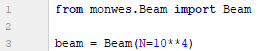
\includegraphics[width=.4\textwidth]{Immagini/Chapter3/BeamRays}
%
\caption{Example of Beam initialization}
%
\label{fig: BeamRays}
%
\end{figure}
Defined the Beam with its number of rays it have to choose the spatial and divergence profile. For the spatial profile there are some possibilities that correspond to different geometrical figure such as: rectangular profile, circular profile, Gaussian profile, point wise profile. The default one is the point wise profile, that it is useful for ideal testing, obviously, for this case,there is no input parameter. All the other profile are characterized by external input in order to define the profile depending on the nature of the profile. for the Gaussian profile the parameter needed is the $\sigma_x $ and  
$\sigma_z $ that correspond the the $\sigma $ of the two dimension, Figure \ref{fig: CodeGaussian} show a code example to define a Gaussian spot of a Beam having $25*10^3 $rays with the two $\sigma $ different, $\sigma_x = 0.1mrad, \sigma_z = 1mrad $ as it is showed in Figure \ref{fig: PlotGaussianExample}.
%
\begin{figure}[H]
%
\centering
%
\subfloat[][Example code for a Gaussian source in spatial coordinate\label{fig: CodeGaussian}]
   {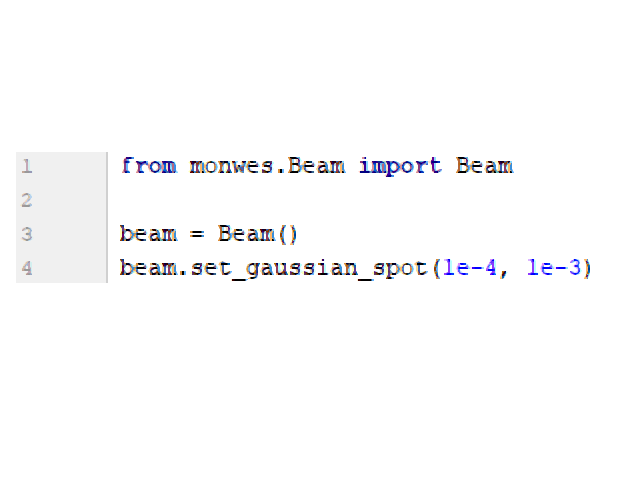
\includegraphics[width=.4\textwidth]{Immagini/Chapter3/GaussianSpot}}\quad
%
\subfloat[][Plot of Figure \ref{fig: CodeGaussian}\label{fig: PlotGaussianExample}]
   {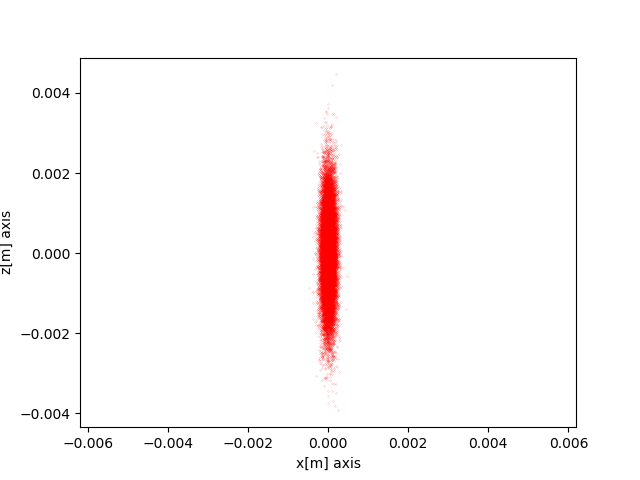
\includegraphics[width=.4\textwidth]{Immagini/Chapter3/GaussianExamplePlotSpot}}
%
\caption{Example 1}
\label{fig :p1}
%
\end{figure}
Over the Gaussian profile, there are other two geometrical profile that can be defined rectangular and circular that have a uniform distribution, of the rays, in their space domain. For the rectangular distribution the parameter to define are the xz limit of the coordinate that define the sides of the rectangle. Figure \ref{fig: CodeRectangleCircle} show an example code where it is defined a circular profile with a radius of 1cm and, after, overwritten another geometrical profile having a rectangular shape, in this case the final profile of the Beam is that figured out in Figure \ref{fig: PlotRectangleExample}, a rectangular non symmetric profile with the coordinate defined in the code in Figure \ref{fig: CodeRectangleCircle}.
%
\begin{figure}[H]
%
\centering
%
\subfloat[][Example code for a circular and a rectangular spot\label{fig: CodeRectangleCircle}]
   {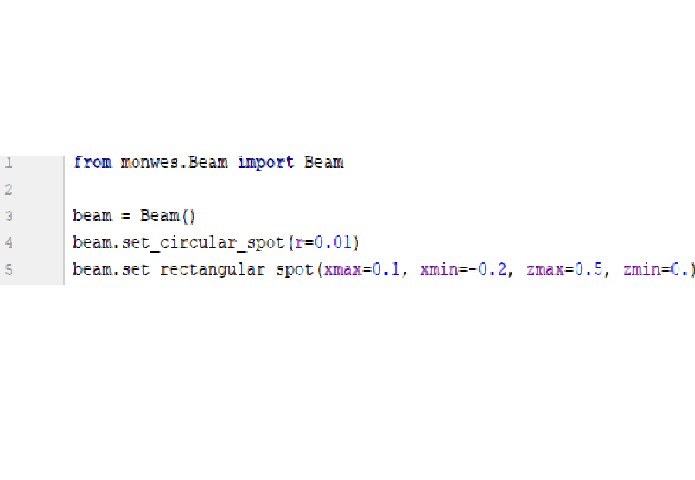
\includegraphics[width=.4\textwidth]{Immagini/Chapter3/CodeCircularRectangular}}\quad
%
\subfloat[][Example plot of the rectangular profile\label{fig: PlotRectangleExample}]
   {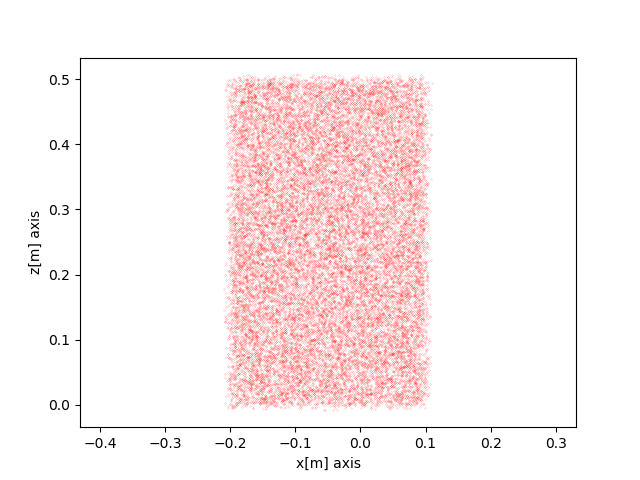
\includegraphics[width=.4\textwidth]{Immagini/Chapter3/RectangularExamplePlotSpot}}
%
\caption{Example 2}
\label{fig :p2}
\end{figure}
Moreover it is possible to define a special shape that have, more or less, the figure of a person with a uniform distribution of the point in all the point of the space. This special shape is showed in Figure \ref{fig: PersonShape}, that is defined in the code written in Figure \ref{fig: CodePerson}. It is used to do a test "imaging" of a system checking that the image, after the optical system, is affected by deformation or defect. As it is showed, the initialize\_ as\_ person command take two input parameter, the number of the total rays (by default are $25*10^3 $), and a size parameter that set the coordinate limit of the figure, more precisely. In Figure \ref{fig: PersonShape} the size correspond to $10^{-6} $ so the limit are: $x_{max} =  1\mu m $, $x_{min} = -1\mu m $, $z_{max} = 1\mu m $, $z_{min} = - 20\mu m $.
\begin{figure}[H]
%
\centering
%
\subfloat[][Example plot "person" profile\label{fig: PersonShape}]
   {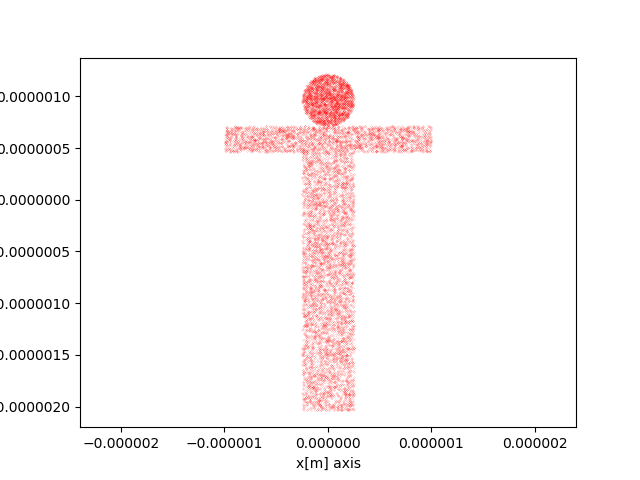
\includegraphics[width=.4\textwidth]{Immagini/Chapter3/PersonExamplePlotSpot}}\quad
%
\subfloat[][Example code for the "person" spot\label{fig: CodePerson}]
   {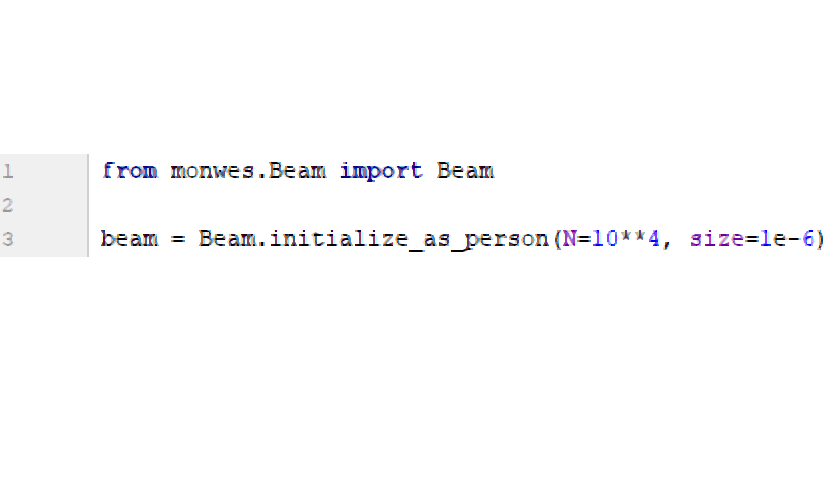
\includegraphics[width=.4\textwidth]{Immagini/Chapter3/CodePerson}}
%
\caption{Example 3}
\label{fig :p3}
\end{figure}
The last piece of the Beam object is the "Flag" vector. Every component of this vector have a correspondence with a certain ray and contain the information about the number of optical element that, the ray, travel until a particular moment. Moreover this value become negative when the ray doesn't hit an optical element, in such a way to have an information where the rays were lost. Figure \ref{fig: ResumeBeam}, resume the main parameter of the Beam object with their default values
\begin{figure}[H]
%
\centering
%
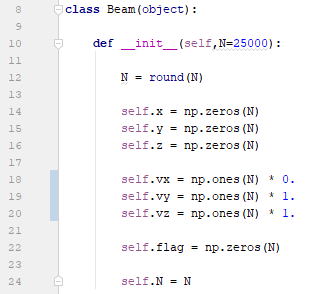
\includegraphics[width=.4\textwidth]{Immagini/Chapter3/ResumeBeam}
%
\caption{Summary of the Beam object parameter}
%
\label{fig: ResumeBeam}
%
\end{figure}
A part from the principal characteristic treated above, Beam object contain other option in order to manage better the utilization of it. The other option defined are reported here below:
\begin{itemize}
\item import\_ from\_ file(filename='filename'): define a Beam with a characteristic defined in a file '.h5'
\item set\_ point(x,y,z): move the Beam in a part of the space centred in the coordinate (x,y,z)
\item initialize\_ from\_ arrays(x, y, z, vx, vy, vz, flag): define a Beam with the spatial value defined in the array x,y,z, the velocities' value defined in the array vx,vy,vz and the flag value defined in the array flag
\item duplicate(): duplicate a Beam
\item good\_ beam(): define a Beam that, starting from another Beam, extract only the good rays (those that have a positive flag)
\item part\_ of\_ beam(indices): define a Beam that, starting from another Beam, extract the ray that correspond to the position defined in the array indices
\item number\_ of\_ good\_ rays(): return the values of the good rays
\item merge(beam2): merge a beam1 with another beam2, the first part of this new beam correspond to the beam1, and the second part to the beam2
\item retrace(distance): this correspond to a free propagation in the space of the Beam within a distance equal to "distance" 
\end{itemize}
At the end there are the command that plot the various characteristic of the beam, that contain the information for the plotted characteristic, for example plot\_ xy() make a plot of the x and y coordinate of the beam, plot\_ good\_ xpzp() make a plot of the x-velocities and z-velocities of only the rays that have a positive flag


\section{Optical Elements}
Because, as discussed in Chapter \ref{Introduzione}, mirrors are the principal elements used in synchrotron the main optical element developed is the mirror, but it is also defined an ideal lens that is useful to simulate some particular profile for the Beam.that corresponding to this , more attention is focused on them, on the contrary , for testing uses, only one kind of lens, an ideal lens, is implemented. 
\subsection{Mirrors and lens}
The different kind of mirror that are defined are:
\begin{itemize}
\item plane mirror
\item sphere mirror
\item ellipsoidal mirror
\item paraboloidal mirror
\item hyperboloidal mirror
%
\end{itemize}
All those geometrical shape are a subset of a surface conical figure. As is discussed in Chapter 2, and reported in Equation \ref{eq: SurfaceConic}, a surface conic is defined by a series of coefficient.
\begin{equation}
a_0 x^2 + a_1 y^2 + a_2 z^2 + a_3 xy + a_4 yz + a_5 xz + a_6 x + a_7 y + a_8 z + a_9 = 0 
\label{eq: SurfaceConic}
\end{equation}
%
The parameter needed to define the correct surface conic shape that define uniquely the mirror desired are:
%
\begin{itemize}
\item focal distances
\item angle of incidence $\theta_g $, more precisely the program use the complementary angle of $\theta_g $ that is $\theta = \frac{\pi}{2} - \theta_g $ (the input and output angle are in radiant)
\end{itemize}
%
Moreover, the surface conic, is defined in such a way to have the origin equal to the incidence point of a collimated ray distant p (that correspond to the object focal distance) from the mirror, and with the normal of the surface corresponding to the z-axis, as it is showed in Figure \ref{fig: ellipse}.
For the plane mirror the situation is simple, because the equation of the surface is that in Equation \ref{eq: PlaneMirror}, that have all the coefficient equal to $0 $ apart from $a_8 $ that is equal to $1 $. 
%
\begin{equation}
z = 0
\label{eq: PlaneMirror}
\end{equation}
%
\\
For the spherical case, the parameter that characterize a sphere is the radius, one time defined the radius, the equation of the sphere is:
\begin{equation}
x^2 + y^2 + z^2 = r^2
\label{eq: sphere}
\end{equation}
Moreover, it is known, from the spherical lens optics (see Chapter \ref{capitolo2}) , that:
\begin{equation}
\frac{1}{p} + \frac{1}{q} = \frac{2}{r_t \sin \theta_g}
\label{eq: sphereLaw1}
\end{equation}
and
\begin{equation}
\frac{1}{p} + \frac{1}{q} = \frac{2 \sin \theta_g}{r_s}
\label{eq: sphereLaw2}
\end{equation}
where $r_t $, is the tangential radius, and $r_s $ is the saggital radius. The sphere case have $r_t = r_s $, this mean that, apart from the normal incidence case, the sphere cannot perfectly focalize/collimate a beam.The radius chosen in Surface\_ conic object is that corresponding to the equation \ref{eq: sphereLaw1}: 
\begin{equation}
r = \frac{2}{\sin \theta_g} \frac{pq}{p + q}
\end{equation}
where p correspond to the object focus length, q to the image lengths, $\theta_g $ to the incidence angle.
\\
For the paraboloid shape, to find the correct coefficients that define the right surface, it is needed the incidence angle, one focal distance and another parameter that distinguish between the two behaviour of the mirror that are showed in Figure \ref{fig: ParabolaFocus} and, Figure \ref{fig: ParabolaColl}. This two system correspond mirrors that, physically, have different behaviour, the first one Figure \ref{fig: ParabolaFocus}, focalize a Beam, the second one, Figure \ref{fig: ParabolaColl}, collimate a Beam.
\begin{figure}[H]
%
\centering
%
\subfloat[][Focalizing case\label{fig: ParabolaFocus}]
   {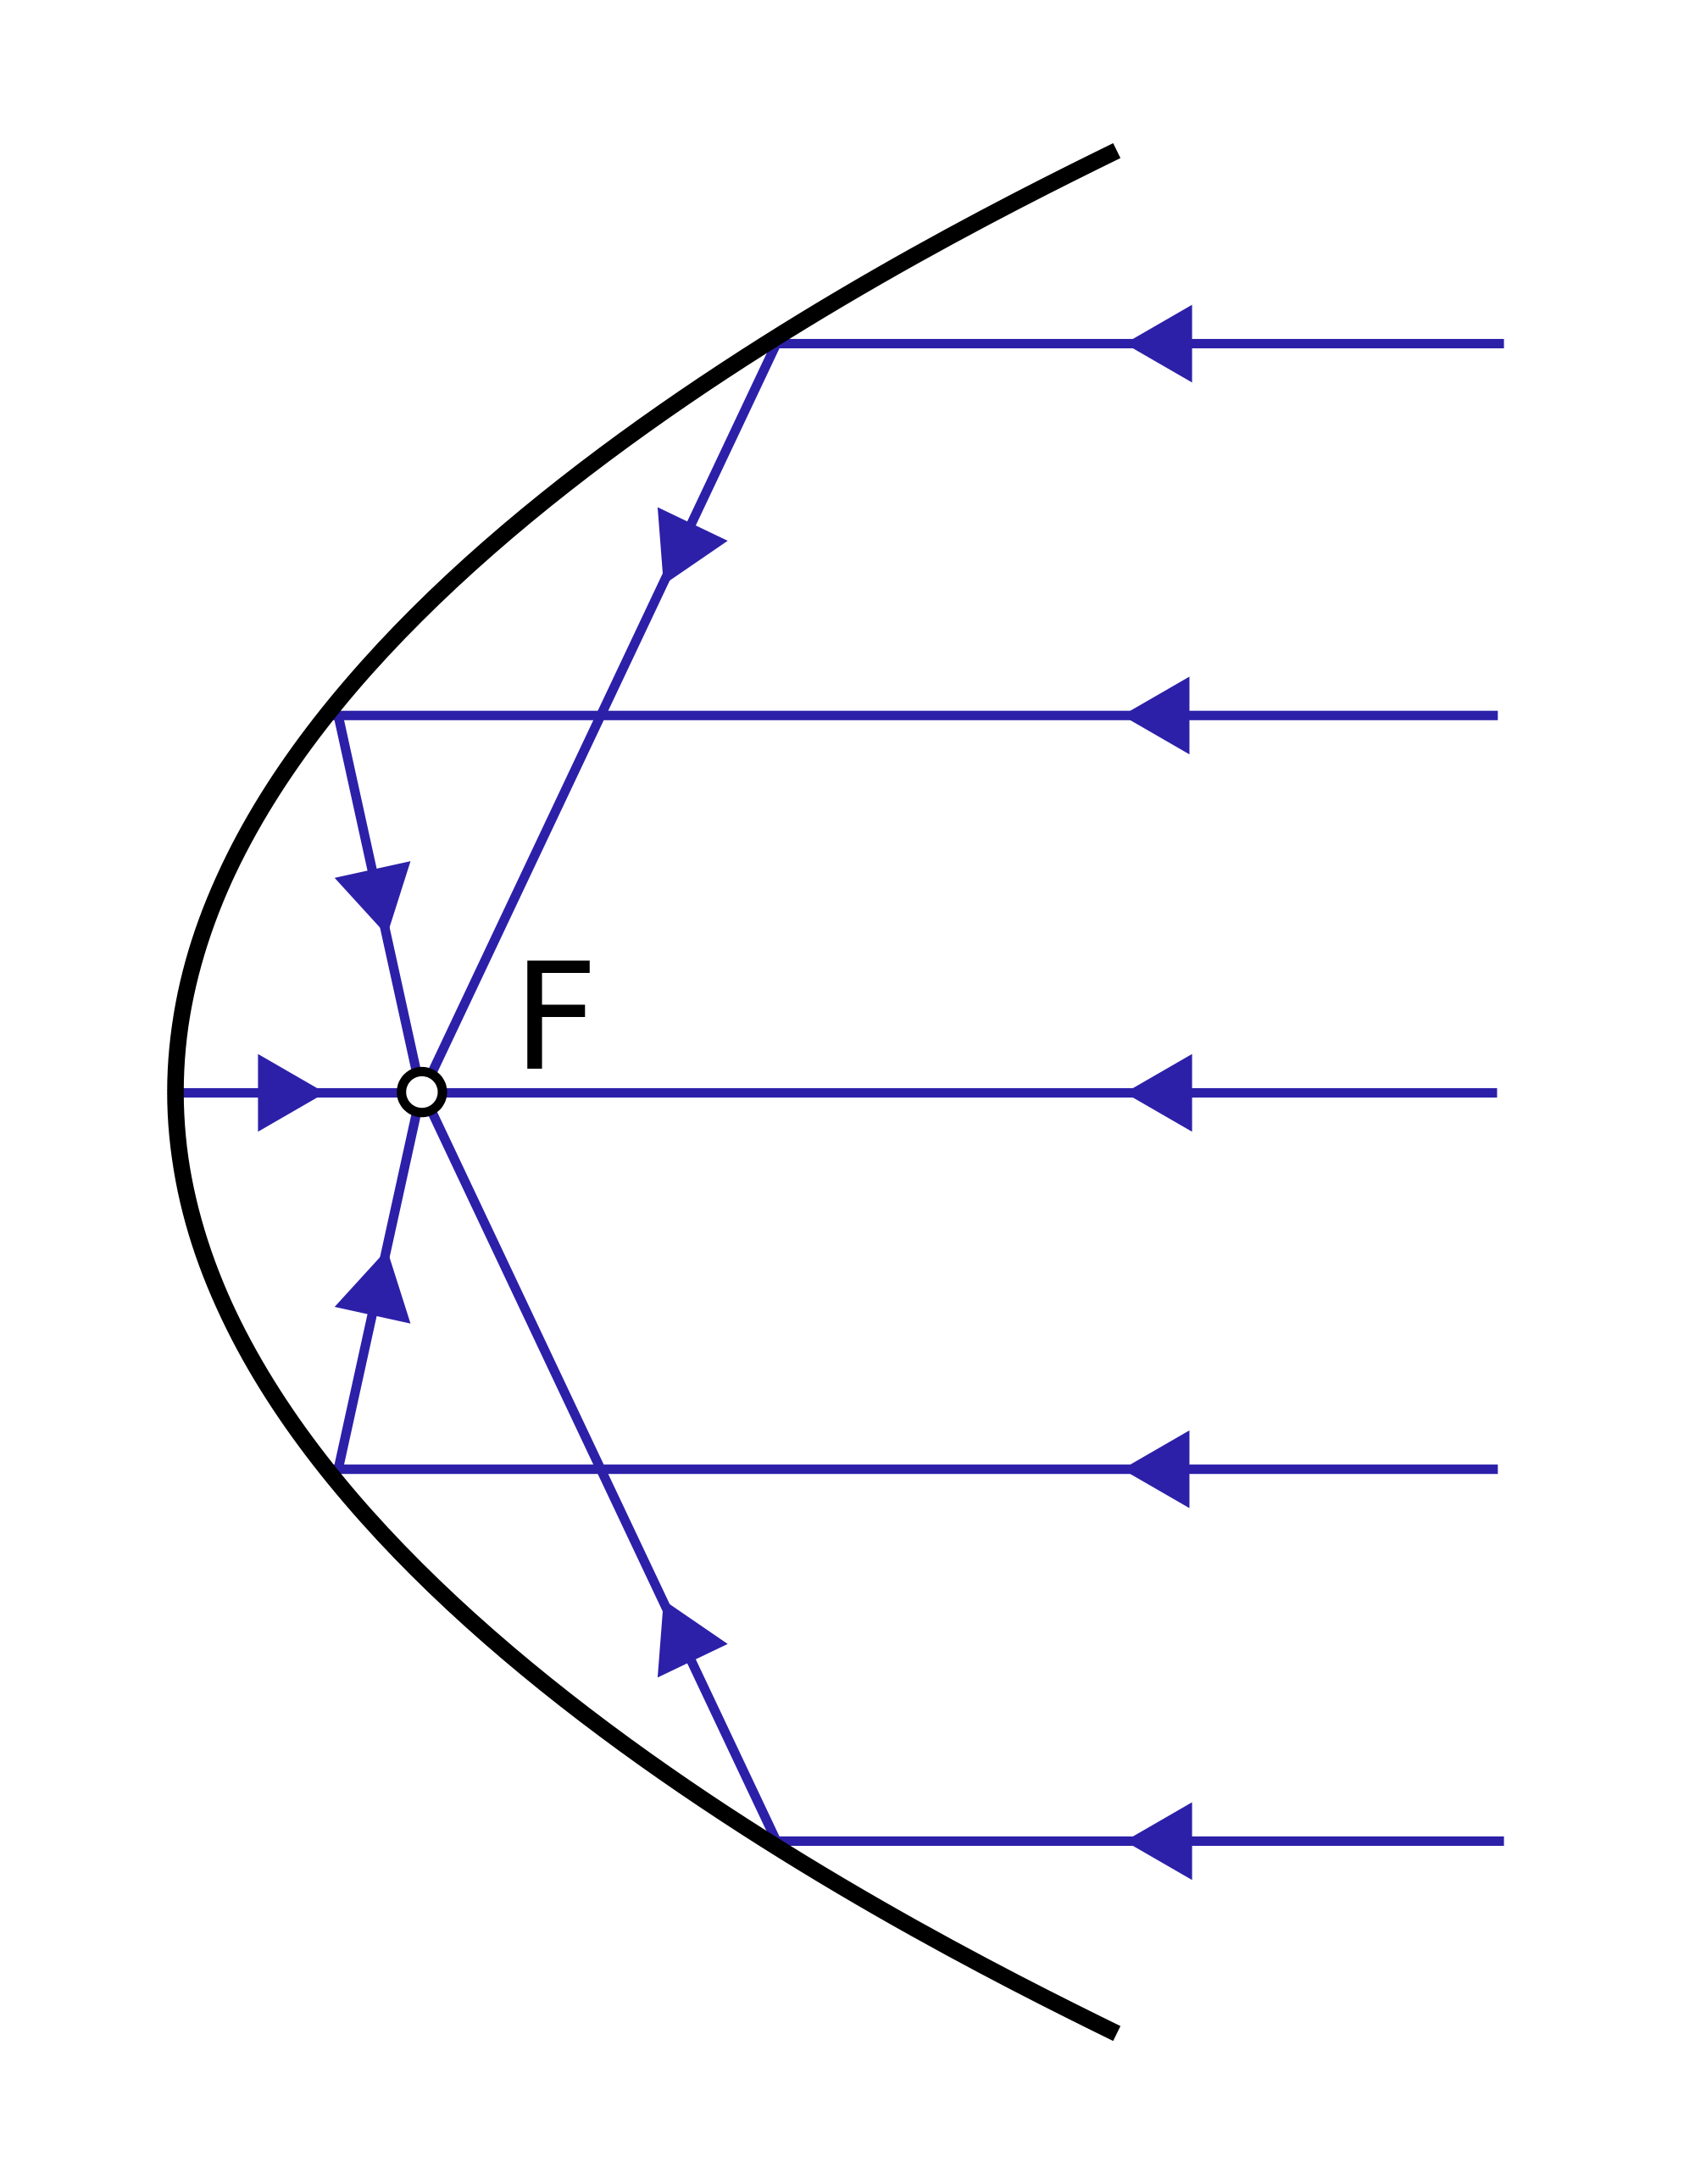
\includegraphics[width=.4\textwidth]{Immagini/Chapter3/ParabolaFoc}}\quad
%
\subfloat[][Collimating case\label{fig: ParabolaColl}]
   {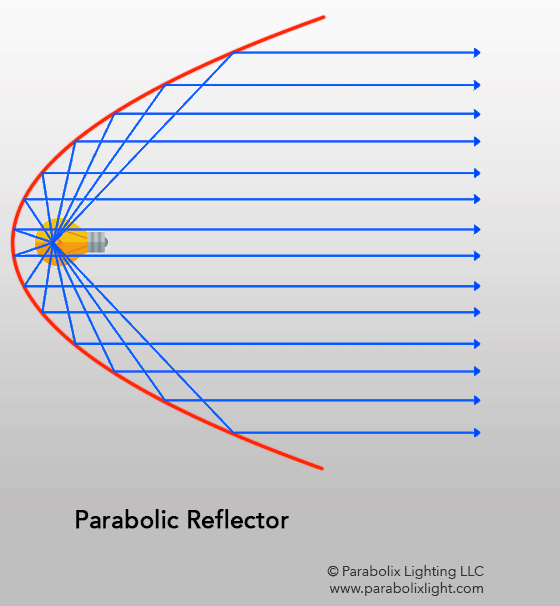
\includegraphics[width=.4\textwidth]{Immagini/Chapter3/ParabolaColl}}
%
\caption{Parabola}
\label{fig :p3}
\end{figure}
The general equation of a parabola, such that in  Figure \ref{fig: ParabolaSystem} is
%
\begin{equation}
y = \frac{1}{4f} x^2
\label{eq: parabola}
\end{equation}
%
where $f $ is the focal distance of the parabola. After a few calculation, see Appendix \ref{cap:AppendixB}, it is possible to correlate $f $ with the input parameter in this sense
%
\begin{equation}
f = d \sin^2 \theta
\label{eq: parabola2}
\end{equation}
%
where d is the object focal distance, in the case depicted in Figure \ref{fig: ParabolaFocus}, otherwise, in the case depicted in Figure \ref{fig: ParabolaColl}, d is the image focal distance.
%
\begin{figure}[H]
%
\centering
%
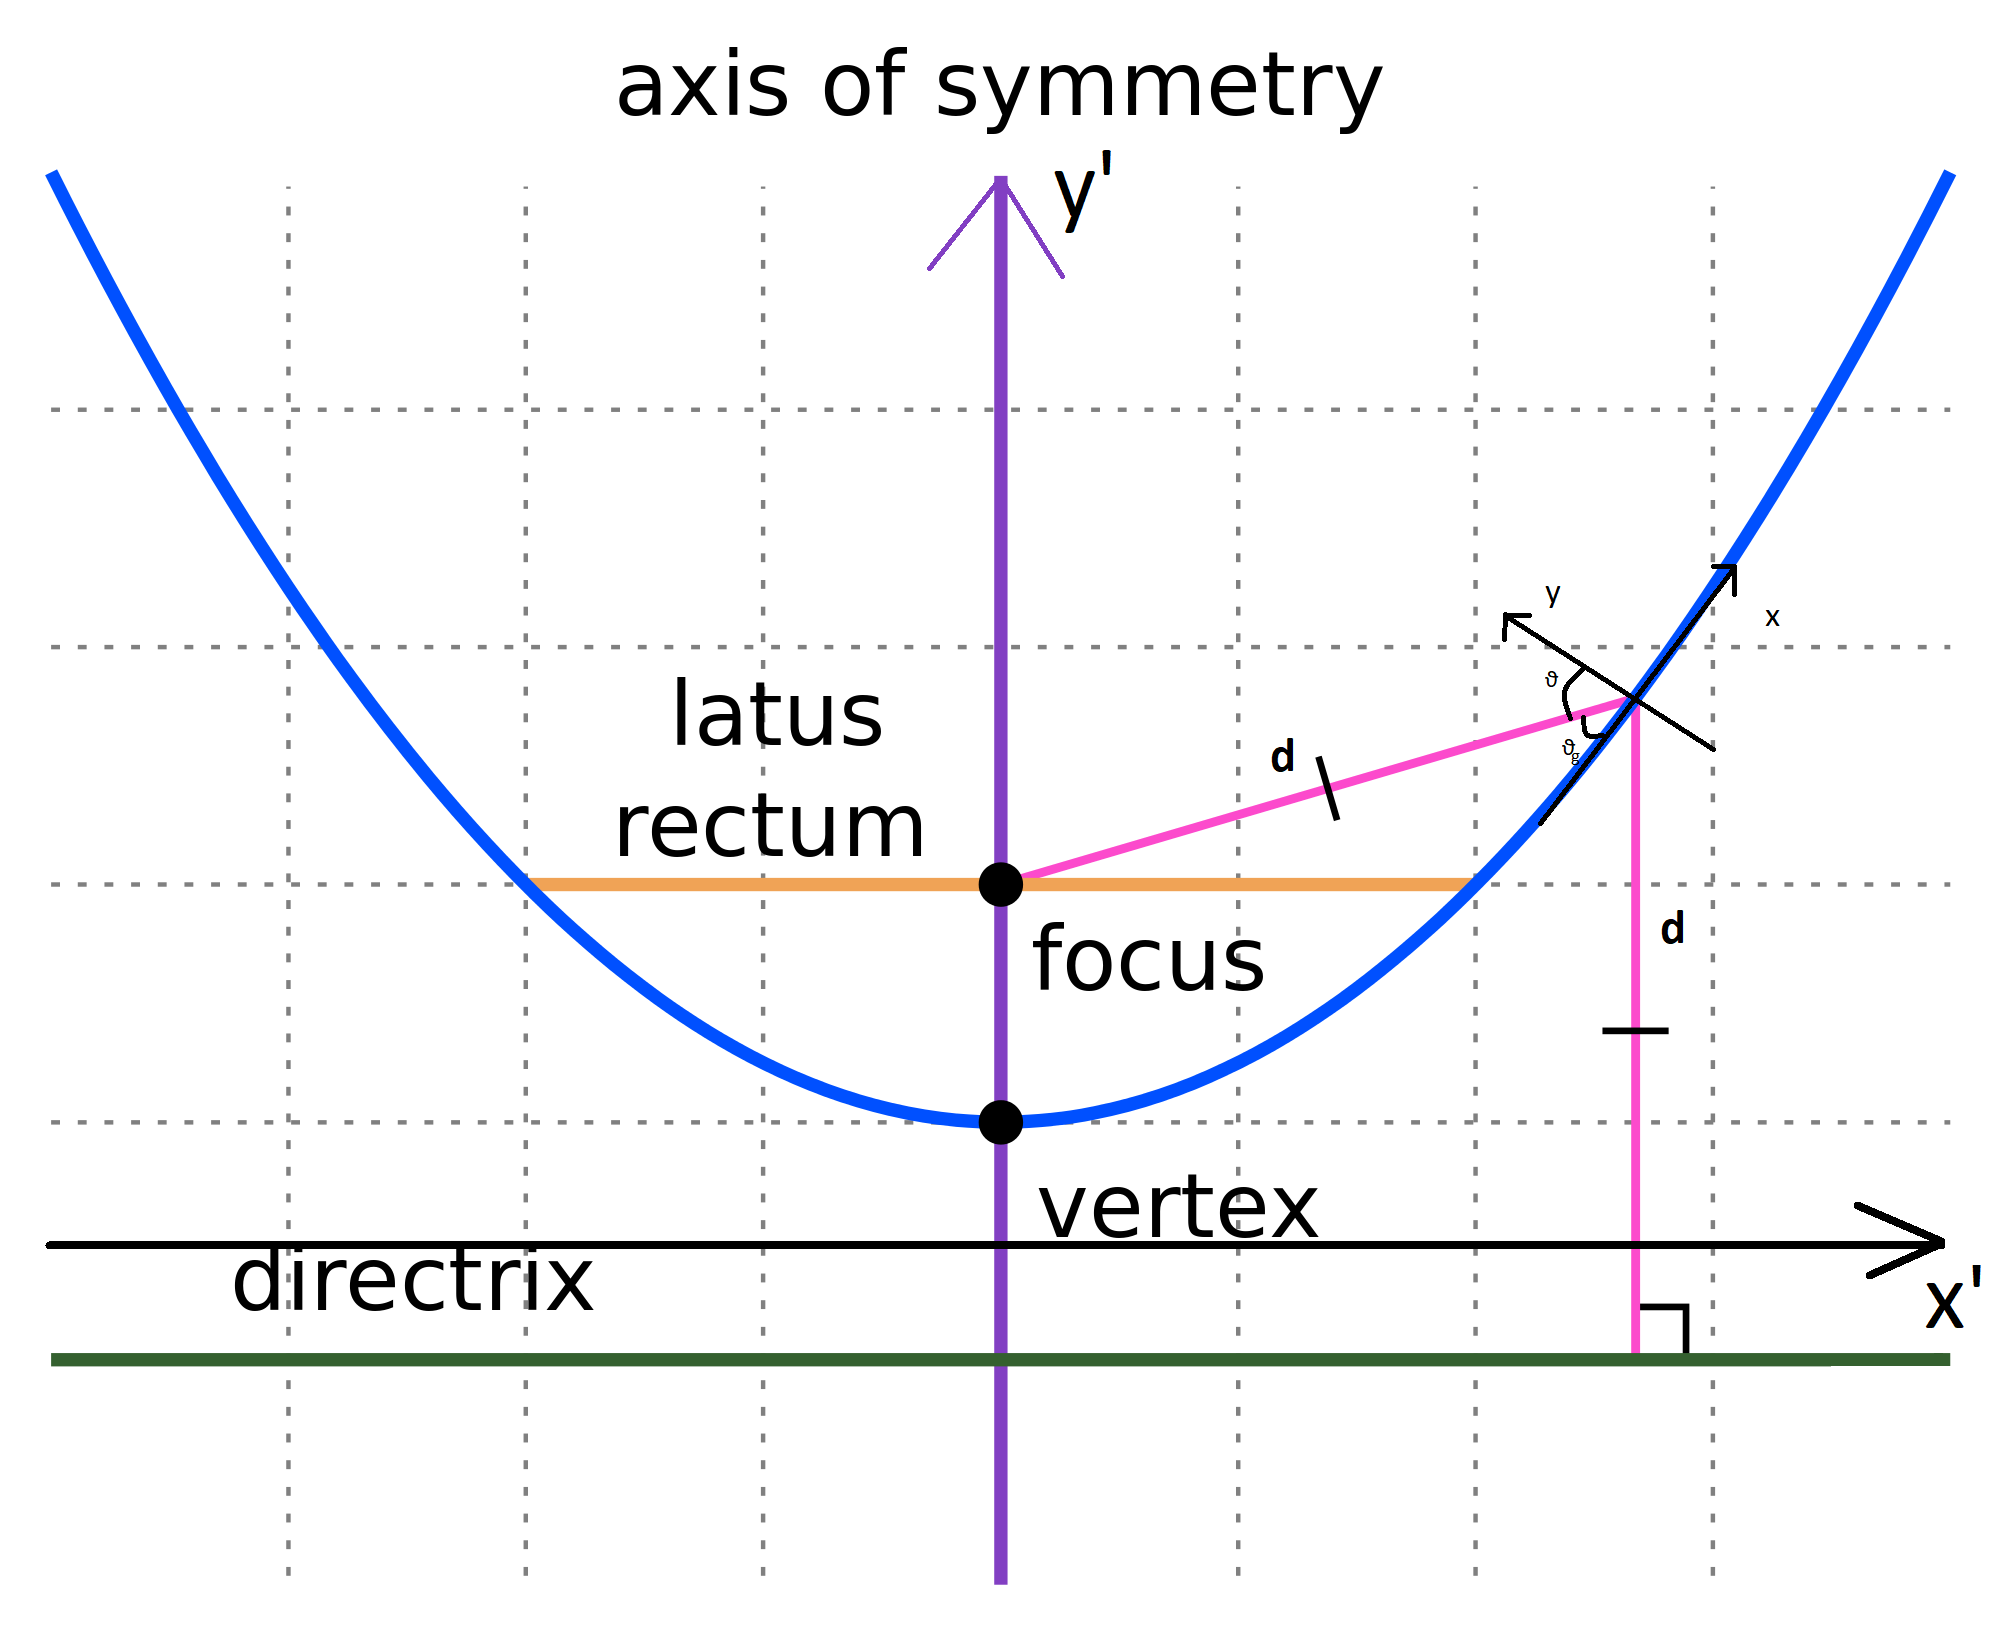
\includegraphics[width=0.8\textwidth]{Immagini/Chapter3/Parab}
%
\caption{System}
%
\label{fig: ParabolaSystem}
%
\end{figure}
For the elliptical case the situation is represents in Figure \ref{fig: ellipse}. Equation \ref{eq: ellipse} describe the general equation of an ellipse where appear two unknown $a$ and $b $.
%
\begin{equation}
\frac{x^2}{a^2} + \frac{y^2}{b^2} = 1
\label{eq: ellipse}
\end{equation}
%
It is possible to correlate (Appendix \ref{cap:AppendixB}), the focal distances plus the incidence angle with the two parameter$a$ and $b $ with the following two equations:
%
\begin{equation}
p = \frac{a + b}{2}
\label{eq: 1stEllipseEq}
\end{equation}
%
\begin{equation}
q = \sqrt{ab} \cos\theta
\label{eq: 2ndEllipseEq}
\end{equation}
%
\begin{figure}[H]
%
\centering
%
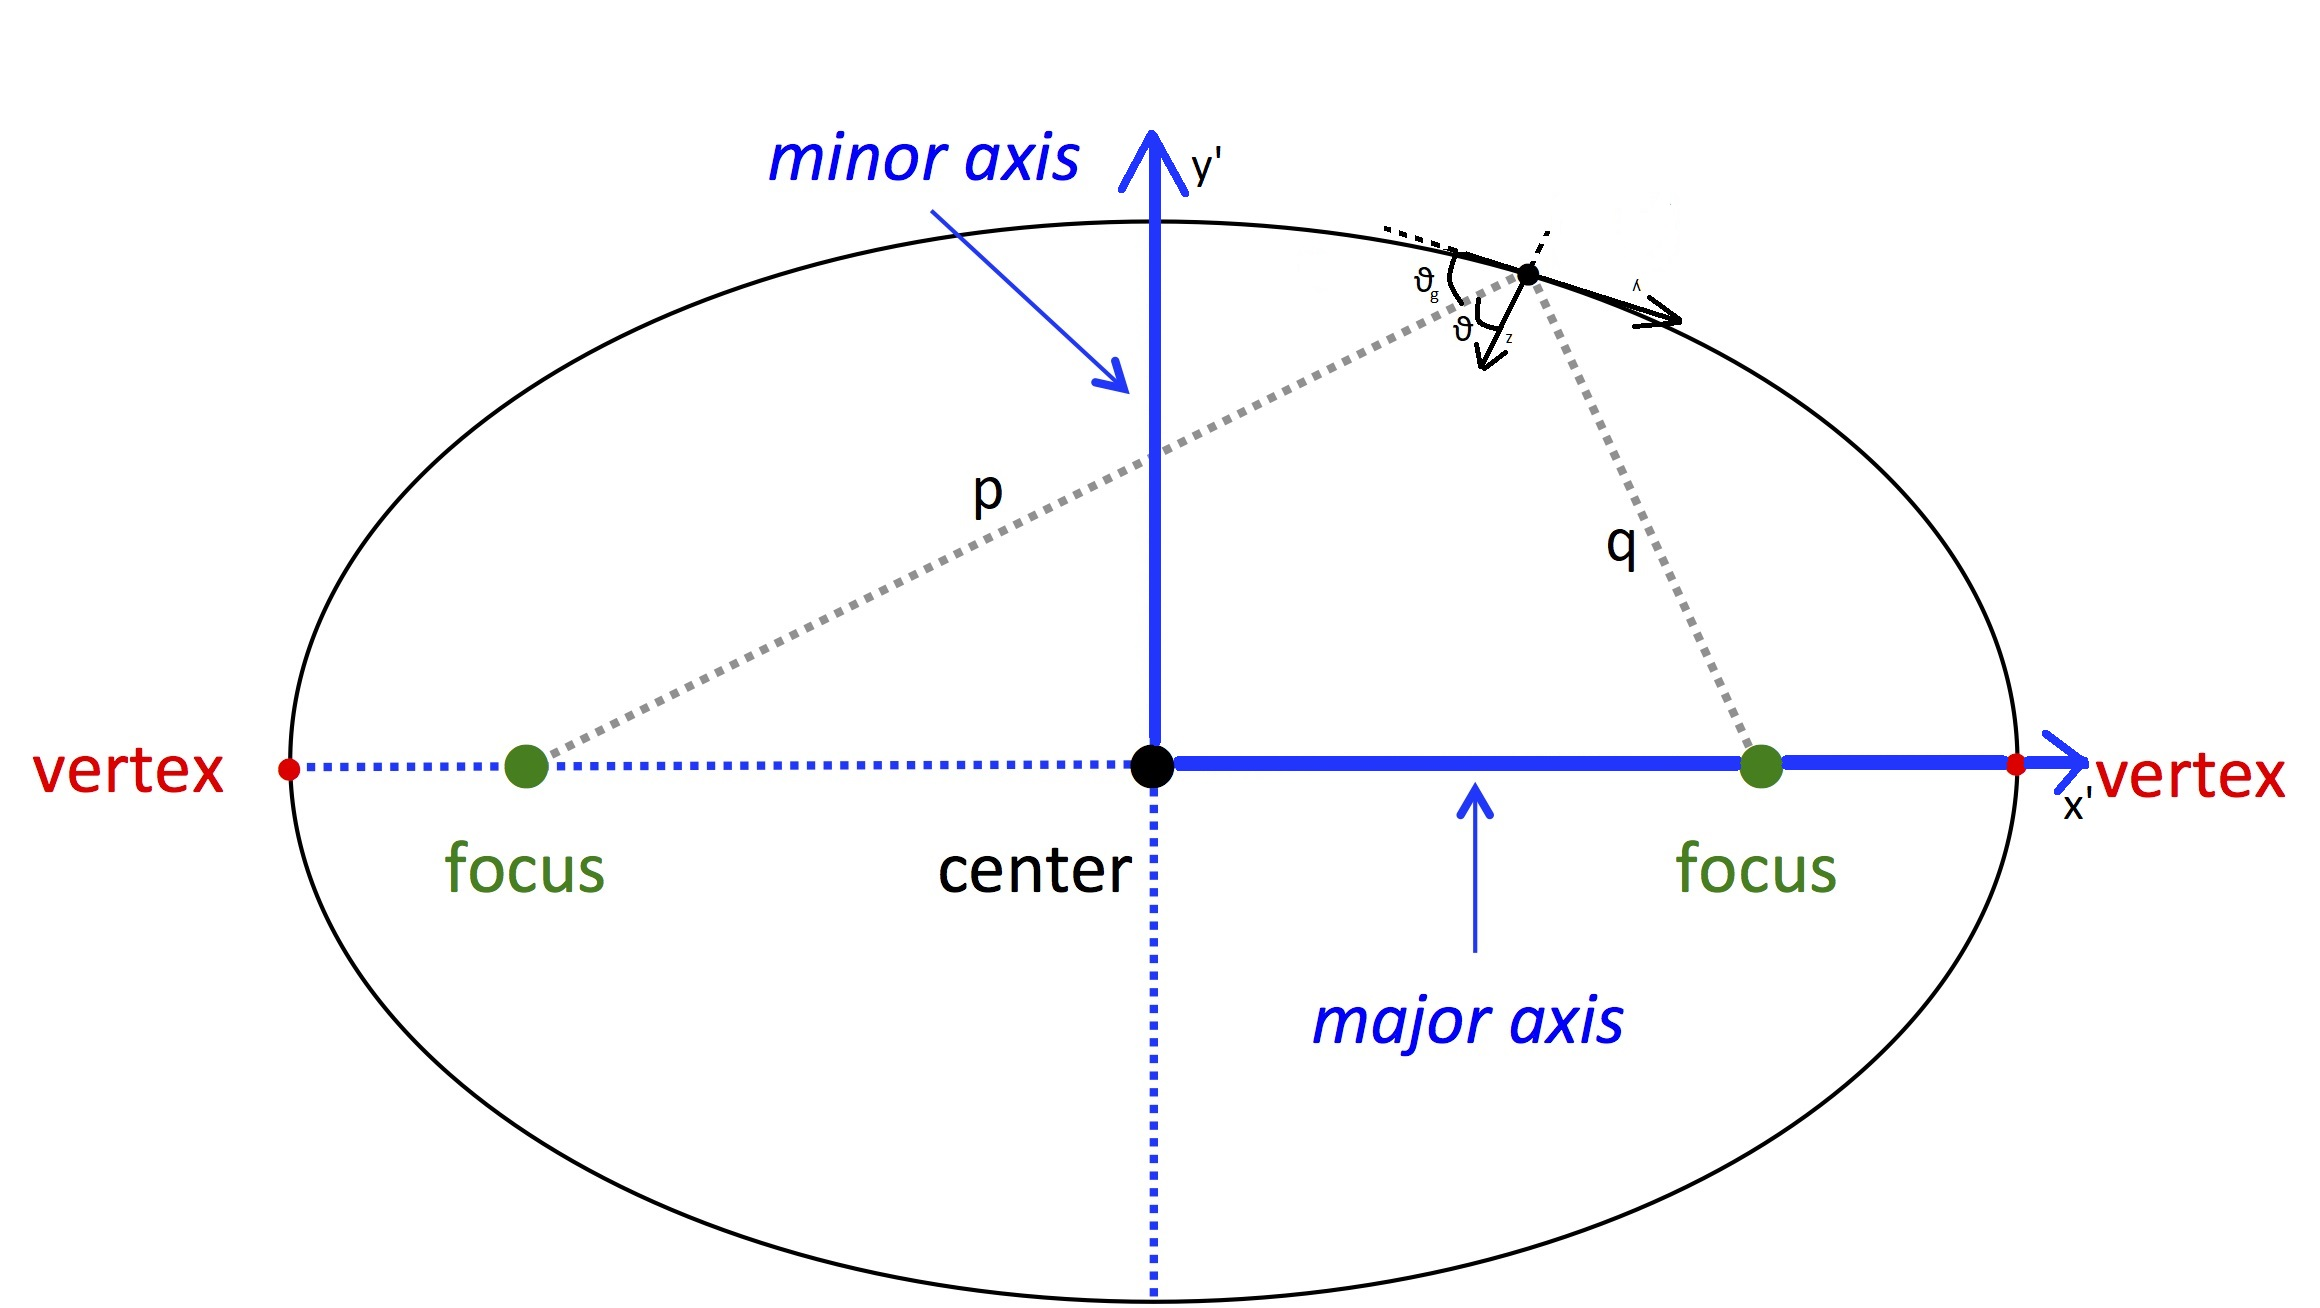
\includegraphics[width=.8\textwidth]{Immagini/Chapter3/EllipseSystem3}
%
\caption{Ellipse System}
%
\label{fig: ellipse}
%
\end{figure}
%
Defined the surface in the $x^{'}y^{'} $, it is done a rotation and a translation in order to center the new $xy $ system on the point P with the normal at that point equal to the z-axis.
\\
For the hyperboloidal mirror the situation is similar to that of the ellipsoidal case, in fact, the general equation of the an hyperbola such the one in Figure is 
%
\begin{equation}
\frac{x^2}{a^2} - \frac{y^2}{b^2} = 1
\end{equation}
%
and the equations that correlate the focal distances and the incidence angle with the parameter $a $ and $b $ are
%
\begin{equation}
p = \frac{a - b}{2}
\label{eq: 1stHypEq}
\end{equation}
%
\begin{equation}
q = \sqrt{ab} \sin\theta
\label{eq: 2ndHypEq}
\end{equation}
%
\begin{figure}[H]
%
\centering
%
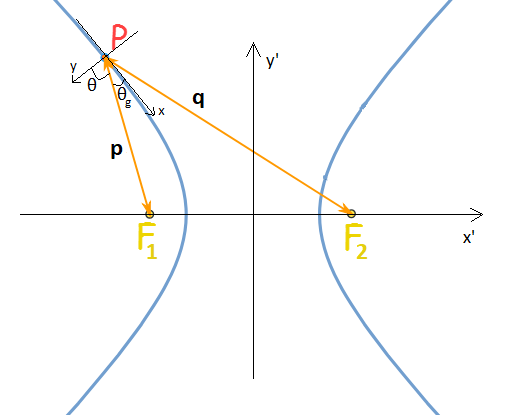
\includegraphics[width=.5\textwidth]{Immagini/Chapter3/Hyperbola}
%
\caption{Hyperbola System}
%
\label{fig: hyperbola}
%
\end{figure}
%
After that it, as in the case of the ellipsoidal mirror, it need a rotation and a translation to complete the work.
For the mirrors, in the program, there is a further option that make the mirror cylindrical in one dimension maintain its surface conic in the other, to do this, in Surface\_ conic object, it is defined a function set\_ cylindrical, that change the shape of the surface, from a complete surface conic, to a surface conic in one dimension and cylindrical in the other.
\\
Apart of the mirrors elements is implement also an ideal lens element that follow the typical lens equation:
\begin{equation}
		\frac{1}{f_x} = \frac{1}{p} + \frac{1}{q}
		\label{eq: lens equation1}
\end{equation}
\begin{equation}
		\frac{1}{f_z} = \frac{1}{p} + \frac{1}{q}
		\label{eq: lens equation2}
\end{equation}
where $f_x $ is the x focal length and $f_z $ is the z focal length. For this optical element the input parameters are the object focal distance, image object distance and the two focal distances ($f_x $, $f_z $) that, in the default mode, are set equal with a value equal to $f_x = f_z = \frac{pq}{p+q} $.

\subsection{Compound Optical Element (KB and Montel system)}

This program include also two different system composed by more mirrors. Starting from conical mirrors, combining them, is possible to have a compound optical elements that can simulate the behaviour of some typical instrumentation that characterize the facilities, in particular in the synchrotron world. The compound optical system implemented are two of those mentioned in Chapter 2:
\begin{itemize}
\item KirkPatrickBaez system (KB system)
\item Montel
\end{itemize}

%\subsection{KirkPatrickBaez System}
KirkPatrickBaez or, more simply, KB system are shown in Figure \ref{fig: KB} is composed by two cylindrical surfacing conic mirror placed one after the other with the two focal lens that converge in the same point. There are implemented two different kind of KB system, a first one composed by two elliptical mirrors and a second one composed by parabolic mirrors. The input parameter that the program need are the two incidence angle and the two focal, with respect to the center of the KB system, represented in Figure \ref{fig: KB1} and the separation of the two mirror, from center to center.
\begin{figure}[H]
%
\centering
%
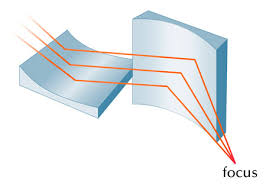
\includegraphics[width=.4\textwidth]{Immagini/Chapter3/KB}
%
\caption{System}
%
\label{fig: KB}
%
\end{figure}
\begin{figure}[H]
%
%\centering
%
\includegraphics[width=.8\textwidth]{Immagini/Chapter3/KB1}
%
\caption{System}
%
\label{fig: KB1}
%
\end{figure}
%%%%%%%%%%%%%%%%%%%%%%%%%%%%%5
%\begin{figure}[H]
%
%\centering
%
%\subfloat[][Focalizing case\label{fig: KB}]
%   {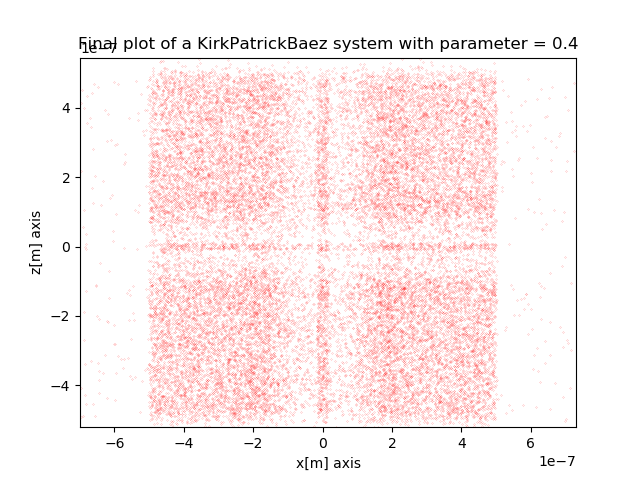
\includegraphics[width=.4\textwidth]{Immagini/Chapter4/KB}}\quad
%
%\subfloat[][Collimating case\label{fig: KB1}]
%   {\includegraphics[width=.4\textwidth]{Immagini/Chapter4/KB1}}
%
%\caption{KB system}
%\label{fig :p5}
%\end{figure}
Because this system is simply a system composed by two surface conical mirror in series the parameter that the system need to define the mirror are not the ones defined by the user but are the focal distance of the two mirrors that are, as shown in Figure, p1, q1, p2, q2, These parameter represent the object focal distance (p1, p2) and the image focal distances (q1, q2) of the two mirror, as represented in Figure \ref{fig: KB1}. Figure \ref{fig: CodeKB}, show an example of the definition for a KB system that have an object focal length of 2m, an image focal distance of 5m, a separation between the two center of the mirrors of 1m, and the two angle of incidence equal each other to $2^{\circ} $.
\begin{figure}[H]
%
\centering
%
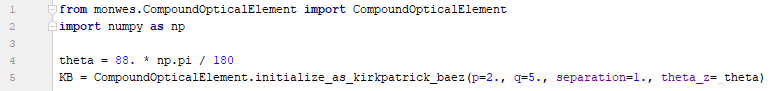
\includegraphics[width=1.\textwidth]{Immagini/Chapter3/CodeKB}
%
\caption{Example 5}
%
\label{fig: CodeKB}
%
\end{figure}
The Montel system, depicted in Figure \ref{fig: MontelSystem}, is composed, as for the KB, by two surface conical mirror cylindrical in one direction, but, because the two mirror are not in series, as for the case of the KB, the situation is a bit complicate. Starting from definition of the two mirrors one is rotated of 90$^\circ $, in order to have a mirror in the xy plane, and another one in the zy plane. As shown in Figure \ref{fig: MontelSystem} the center of the Cartesian system is setted in the point where the  optical axis of the system hit the compound system having the normal of the first normal equal to the z-axis, and the second normal equal to the - x-axis. The system is defined by the following parameter p, q, $\theta_z $, $\theta_x $, where p and q are the focal distance of the two mirrors and $\theta_z $ and $\theta_x $ are the angle of incidence to define the correct mirrors  (by default $\theta_z = \theta_x $).
\begin{figure}[H]
%
\centering
%
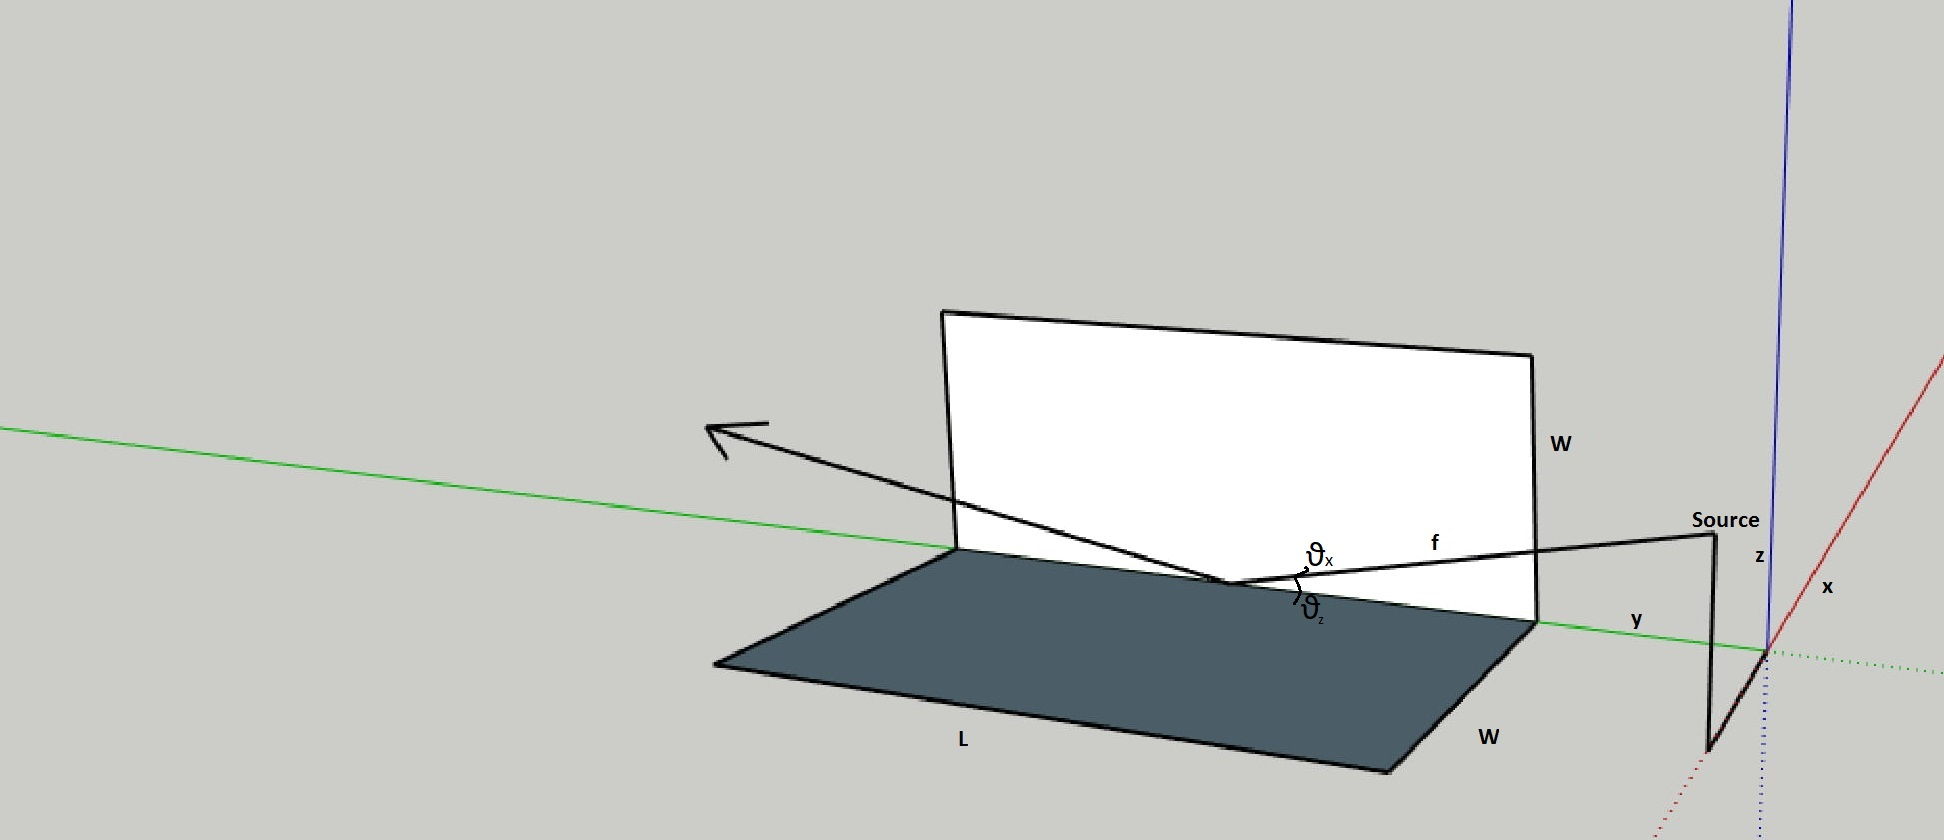
\includegraphics[width=1.\textwidth]{Immagini/Chapter3/MontelSystem2}
%
\caption{System}
%
\label{fig: MontelSystem}
%
\end{figure}
The following Figure \ref{fig: CodeMontel} show an example code for a parabolic Montel system having an object focal length of 5m, image focal length of 2m and the two incidence angle of $1.5^{\circ} $, that focalize a Beam. As for the KB system also in this case there are implemented two possibilities, an ellipsoidal system (having the two mirror as ellipsoid), and parabolic system (having the two mirror as ellipsoid). 
\begin{figure}[H]
%
\centering
%
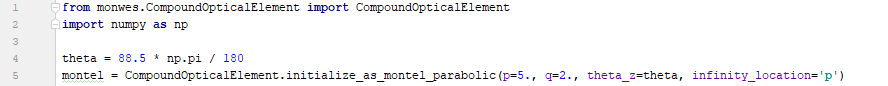
\includegraphics[width=1.\textwidth]{Immagini/Chapter3/CodeMontel}
%
\caption{Example 6}
%
\label{fig: CodeMontel}
%
\end{figure}
%
\section{Tracing System}
Defined the Beam and the different optical element, to complete a simulation, is needed a tool that put everything together and modify the property of the beam after the interaction with the optical elements.
\\
For example, if it want to simulate the system depicted in Figure \ref{fig: System}, it have to define a Beam source, the optical element and, at the end, somewhere, the distances between the optical elements. The tracing part of the program, for the non-compound optical element, is written in such a way that the trace work in series, one optical element after the other. This, in series methods, work with the definition of two distances, object/image distance from the center of the optical element, the incidence angle of the Beam, that can be different from the designing one,and a second angle that define the mirror with respect to the Beam. (normally and also for the default case the incidence angle i equal to the designed one, and the second angle is fixed to $0^{\circ} $). One possibilities, to define the system in Figure \ref{fig: System} is to set the object distances of the mirrors equal to distance $d_0 $ and $d_1 $, and the image distances equal to $0 $, for the lens lets set the object distance equal to $d_3 $ and the image distance equal to $d_4 $ as it is reported in Figure \ref{fig: CodeSystem}.
\begin{figure}[H]
%
\centering
%
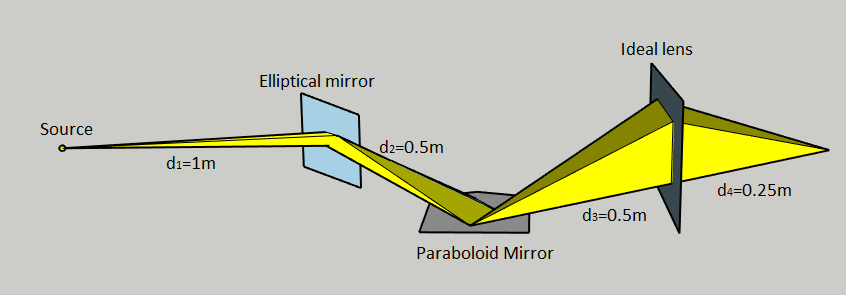
\includegraphics[width=1.0\textwidth]{Immagini/Chapter3/Cattura}
%
\caption{System}
%
\label{fig: System}
%
\end{figure}
\begin{figure}[H]
%
\centering
%
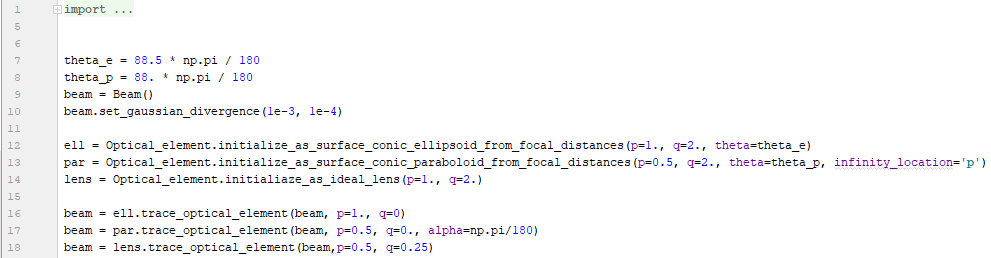
\includegraphics[width=1.\textwidth]{Immagini/Chapter3/CodeSystem}
%
\caption{Example 7}
%
\label{fig: CodeSystem}
%
\end{figure}
%
\subsection{Tracing for simple Optical element}
Going deeper in the code, the algorithm that trace a single element is divided in 5 step
\begin{enumerate}
	\item change the reference system from that of the optical axes to that of the optical element after two rotation, one along x-axis, and second along y-axis, and a translation equal to the object distance of the optical element
	\item free propagation up to the optical element
	\item effect of the optical element
	\item free propagation to the image plane
	\item changing the Cartesian system in that one that have the optical axis equal to the y-axis
\end{enumerate}
The first three point are condensed in the method effect\_ of\_ the\_ optical\_ element, that is showed in Figure \ref{fig: CodeEffOpt}, and the last two point are condensed in the method effect\_ of\_ the\_ screen that is showed in Figure \ref{fig: CodeEffScreen}.
\begin{figure}[H]
%
\centering
%
\subfloat[][Example code for a Gaussian spot\label{fig: CodeEffOpt}]
   {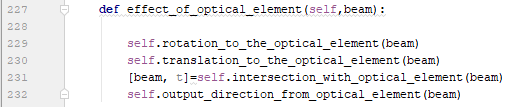
\includegraphics[width=.4\textwidth]{Immagini/Chapter3/CodeOptElem}}\quad
%
\subfloat[][Plot of Figure \ref{fig: CodeGaussian}\label{fig: CodeEffScreen}]
   {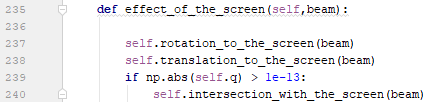
\includegraphics[width=.4\textwidth]{Immagini/Chapter3/CodeOfScreen}}
%
\caption{Example 1}
\label{fig :p1}
%
\end{figure}
Because of the different definition, the tracing method of the rays' beam, need a different interpreter that can link the beam with the different optical elements that meet on his way. Because of the different nature, there are implemented two kind of tracing, a first one that trace the KB system, that is composed by a series of optical elements and so can be used for all the compound optical elements that are in series. And a second one that is specific for the Montel system, because it is not composed by mirrors in series rather than mirrors in parallel, having the two elements in a very small region of the space that have in which order the rays of the beam hit the different mirrors.
\subsection{Tracing for KB}
For KB system the situation is more or less the same as for a simple optical mirrors, with the only difference that there are more than one mirror. So the algorithm to simulate the tracing system is nothing else than a for loop, that use the tracing system of the simple optical element. In this the object and the image distance from the center of the system are the default ones, such as for the incidence angles. Figure \ref{fig: CodeTraceCompund}, show the trace code for the compound elements that are in series.
\begin{figure}[H]
%
\centering
%
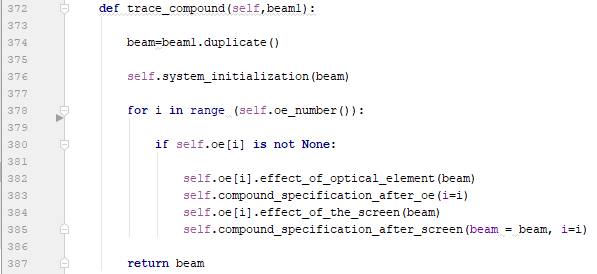
\includegraphics[width=1.\textwidth]{Immagini/Chapter3/CodeTraceCompound}
%
\caption{Example 8}
%
\label{fig: CodeTraceCompund}
%
\end{figure}
\subsection{Tracing for Montel}
Montel system is completely different from the KB system and all the series optical system, so it need a new trace system. This new trace system is divided as follow
\begin{enumerate}
	\item Changing the reference frame in one having the center on the center of the mirrors, with a z-axis corresponding to the normal of one mirror and -x-axis equal to the normal of the second mirror. This transformation is done in a similar way of the normal tracing, two rotation of the beam, and one translation, differently from the normal tracing, the two rotation are done such that the beam hit the mirrors with an incidence angle set by the user
	\item Focus the attention on the travel time of each ray in order to know which is the nearest optical element of each ray
	\item free propagation of each ray up to the nearest optical element
	\item effect of the system for each ray
	\item repeat the 2$^{nd} $, 3$^{rd} $ and 4$^{th} $ passage two times, in order to consider the two reflection
	\item Change the reference system to the optical axes that is subject to two reflection, doing two rotation and one translation
\end{enumerate}  

\noindent What is reported above is the default tracing system that, because of its centrality on my thesis' work have many option. What is set by the user is 
\begin{enumerate}
	\item focal distances and incidence angles, that define the two rotation and the translation of the tracing system
	\item name of the File in which is saved the data of the simulation, by default no data is saved
	\item there is the possibility to choose a different point, from the origin, in which the the optical axis hit the system
	\item there is also the possibility to have a final output frame that is not solidal by the two-reflected beam, but with the non reflected beam or with the other two beam that are reflected only one time
	\item It is also the possibility to figure out the footprint of the two reflected beam on the system. For clarity the beam that hit the first mirror and after the second is labelled with red point, the beam that hit the second and after first mirror is labelled by blue color
\end{enumerate}

\noindent These options are added in order to study better the behaviour of a beam with a Montel system. The possibilities to change the angle of incidence and to hit different part from the origin can be used to study what happen to a beam when is not aligned, or not perfectly aligned, and use these result to align the system in the laboratories. The possibilities to save a File is useful in particular in those case where there is a huge computational effort that need a lot of time, in these cases is possible to work with the result of a big simulation without reappointing it, and so save time. Figure \ref{fig: CodeTraceMontel} show the code that trace a Montel elements, containing also the special option that were defined above.
\begin{figure}[H]
%
\centering
%
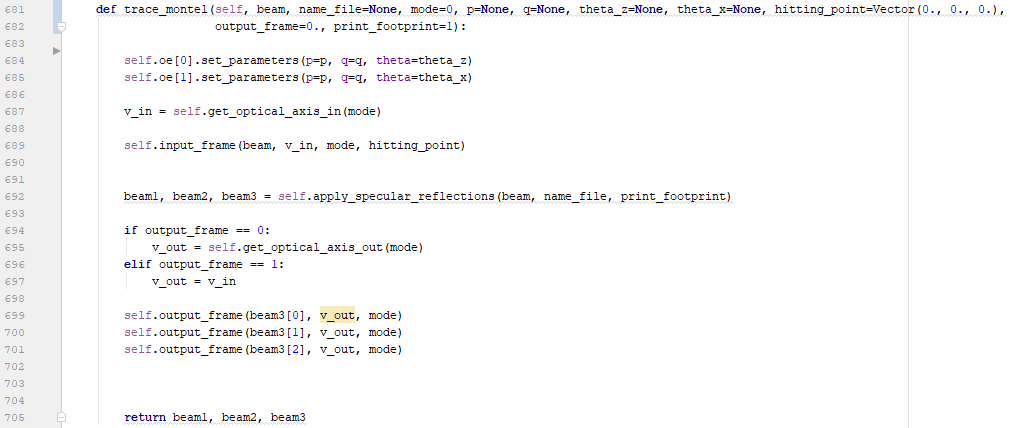
\includegraphics[width=1.\textwidth]{Immagini/Chapter3/CodeTraceMontel}
%
\caption{Example 8}
%
\label{fig: CodeTraceMontel}
%
\end{figure}